\chapter{Conclusions}
\label{sec:concl}
The way malicious nodes disseminate bogus network information makes the attack resemble fake bootstrapping and eclipse attack.

In particular, the adversary exploits \texttt{addr} messages exchanges and their relay policy to extensively disseminate false network information. Most \texttt{addr} messages are exchanged when peers setup connections, thus the attack efficacy is proportional to the number of connections made over time.

On top of that, the adversary takes advantage Bitcoin's unique \texttt{addr} relay policy, that allows to further spread malicious addresses.

The efficacy of the strategy has been proven high, as with just 10\% of the identities on the network the adversary can completely fill peer caches with malicious addresses (Figure~\ref{fig:avgatk-known}). Moreover, attackers are highly connected with honest nodes (Figure~\ref{fig:avgatk}.

The Sybil attack executed on the new overlay network is substantially more powerful, as it makes coverage drop steeply with less malicious nodes involved in the attack (Figure~\ref{fig:in-cov}).

It is necessary to point out that the new Sybil attack achieves high efficacy despite working with a network far more dense than the one in the results of Serena et al (Figure~\ref{fig:degreehon}). Their work assessed the importance of an highly connected graphs as a direct countermeasure to Sybil attacks of this kind.

Therefore, the results obtained imply an increased feasibility of the attack, since the adversary needs to control fewer identities to disrupt honest activities. With just the 20\% of the nodes it is possible to make coverage drop below 40\% (~\ref{fig:in-cov}).\par

Nonetheless, the setting of the attack is ideal and cannot be compared to that of a real network. The positive outcome is influenced by the increased capability to spread network information during the time the graph topology is still forming.

Under no circumstances the real Bitcoin network could undergo such process. For this reason the attack has been carried out on a second scenario where all the malicious nodes are on fresh bootstrap.

The results in Figure~\ref{fig:ext-cov} show how the attack was utterly ineffective even though the network was still being built at the time the Sybils started to join.
 
Furthermore, Sybils did not achieve their objective during network creation, since the average percentage of attacking neighbours (Figure~\ref{fig:ex-atk-neigh}) is significantly lower.

Despite that, there is no gap that big in the rate of Sybils in the peer cache (Figure~\ref{fig:ex-atk-known}) between the two attack scenarios, thus stating the attackers could still disseminate rather well their addresses.

This means that the positive outcome of the attack in the first scenario was influenced by two factors: the presence of Sybils in the DNS lists and the time at which malicious addresses start to be disseminated.

Although the first factor has been surely influential in later stages of the simulation, when the number of attackers increased, from Figure~\ref{fig:dns} and~\ref{fig:in-cov} is possible to see how the steep decrease in coverage is not proportional to the increase in the percentage of attackers as DNS seeds.

On the other hand, the reader can now see how timing is essential for the good outcome of the attack, since starting the attack late allows honest nodes to form their own sparse network.

The data in Figure~\ref{fig:beginning}, relative to the first attack scenario, shows the percentage of malicious addresses in peer caches before bootstrapping nodes start to join. In the second scenario, no Sybils can be in any peer cache at the start, since they have to join the network first.\par

\begin{figure}[h!]
	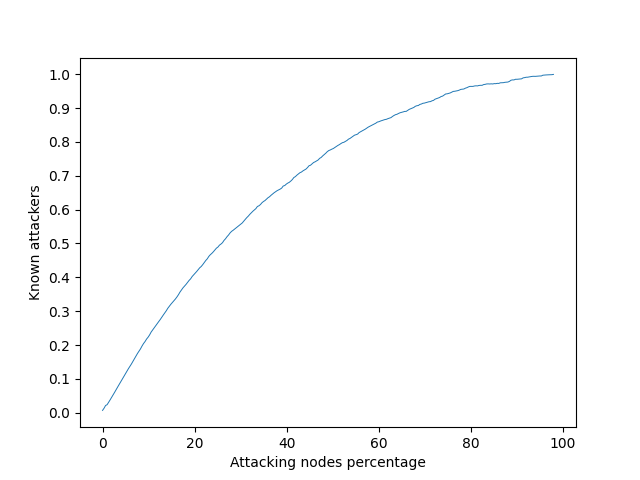
\includegraphics[width=.7\textwidth]{pict/results/in-atkknown-beginning.png}
	\centering
	\caption{Percentage of Sybils in the peer cache at the beginning of the graph construction in the first attack scenario}
	\label{fig:beginning}
\end{figure}

It is evident that honest nodes have a good probability of connecting to malicious nodes as their first or second neighbour, with just a few Sybils in the network.

Whenever this happens their caches are filled with malicious addresses. From that point on the chance of connecting to another malicious address will be extremely high.

For this reason, the sooner a node connects to a malicious address the more likely it is that it will be eclipsed or have an high amount of Sybils amongst its neighbours.

This condition will further enhance the efficacy of the attack from then on: when a honest node connects to another, it is likely that it will send mostly malicious addresses to it, thus helping the adversary disseminating bogus information.

The sooner this chain of exchanges starts, the better for the attacker, as more and more nodes find only malicious addresses in their caches.

Although, the network develops differently in the second scenario. Most of the honest nodes have already at least one honest neighbour at the time malicious nodes start to join. Therefore it is likely that their second neighbour will be another honest node.

This creates a sparse honest-only subgraph that, despite being well connected with the Sybils subgraph, is entirely resistant to the attack.

Moreover, in this phase \texttt{addr} exchanges between honest nodes cannot contain Sybil addresses, as they are bootstrapping. This decreases the probability of connecting to a Sybil as second or third connection, therefore making the honest-only subgraph even more dense.

Lastly, malicious nodes cannot carry out fake bootstrapping, since their addresses are not in DNS lists, and as a result bootstrapping honest nodes will surely contact other honest nodes first.

All of these reasons concurrently hinder the success of the attack. Despite succeeding at disseminating false network information, Figure~\ref{fig:ex-atk-known}, the adversary can never make enough connections with honest nodes (Figure~\ref{fig:ex-atk-neigh}).
Thus, the data from the victim to the rest of the network cannot be blocked.

The result holds even with and extremely large number of Sybils, that in the tests are as much as three times the total of honest nodes.

To conclude, the major factor for the success of the attack was the presence of Sybil nodes in the network before the attack started. This has given a chance to the adversary to get inside DNSs seed lists and to start disseminating false information early on, thus completely changing the way the network forms.

However, it is likely that the attack would not be effective on the real Bitcoin network, since the topology has already formed, connections are set up and peer caches are full of honest nodes. The adversary would have to wait for nodes to leave and join to disseminate bogus data, and try to fake bootstrap unfortunate peers, thus slowing down the set up for the attack. Further work may try to assess the feasibility and efficacy of such attacks on the real Bitcoin network.

Be that as it may, this work has demonstrated how effective disseminating fake network information can be. This is particularly true if the adversary stays in the network long enough, thus disseminating fake information for longer and having a chance to eclipse bootstrapping victims.

The danger of fake bootstrapping for new, isolated nodes is real. An adversary that manages to keep these nodes isolated long enough may create multiple network partitions, or a single, larger partition that can be exploited for selfish mining or N-confirmations double-spending attacks.

New works can focus on an evaluation of the risks of fake bootstrapping for merchants and try to develop new secure means to join a peer-to-peer network. 